%!TEX TS-program = xelatex

% Шаблон документа LaTeX создан в 2018 году
% Алексеем Подчезерцевым
% В качестве исходных использованы шаблоны
% 	Данилом Фёдоровых (danil@fedorovykh.ru) 
%		https://www.writelatex.com/coursera/latex/5.2.2
%	LaTeX-шаблон для русской кандидатской диссертации и её автореферата.
%		https://github.com/AndreyAkinshin/Russian-Phd-LaTeX-Dissertation-Template

\documentclass[a4paper,14pt]{article}

%%% Работа с русским языком
\usepackage[english,russian]{babel}   %% загружает пакет многоязыковой вёрстки
\usepackage{fontspec}      %% подготавливает загрузку шрифтов Open Type, True Type и др.
\defaultfontfeatures{Ligatures={TeX},Renderer=Basic}  %% свойства шрифтов по умолчанию
\setmainfont[Ligatures={TeX,Historic}]{Times New Roman} %% задаёт основной шрифт документа
\setsansfont{Comic Sans MS}                    %% задаёт шрифт без засечек
\setmonofont{Courier New}
\usepackage{indentfirst}
\frenchspacing

\renewcommand{\epsilon}{\ensuremath{\varepsilon}}
\renewcommand{\phi}{\ensuremath{\varphi}}
\renewcommand{\kappa}{\ensuremath{\varkappa}}
\renewcommand{\le}{\ensuremath{\leqslant}}
\renewcommand{\leq}{\ensuremath{\leqslant}}
\renewcommand{\ge}{\ensuremath{\geqslant}}
\renewcommand{\geq}{\ensuremath{\geqslant}}
\renewcommand{\emptyset}{\varnothing}

%%% Дополнительная работа с математикой
\usepackage{amsmath,amsfonts,amssymb,amsthm,mathtools} % AMS
\usepackage{icomma} % "Умная" запятая: $0,2$ --- число, $0, 2$ --- перечисление

%% Номера формул
%\mathtoolsset{showonlyrefs=true} % Показывать номера только у тех формул, на которые есть \eqref{} в тексте.
%\usepackage{leqno} % Нумерация формул слева	

%% Перенос знаков в формулах (по Львовскому)
\newcommand*{\hm}[1]{#1\nobreak\discretionary{}
{\hbox{$\mathsurround=0pt #1$}}{}}

%%% Работа с картинками
\usepackage{graphicx}  % Для вставки рисунков
\graphicspath{{images/}}  % папки с картинками
\setlength\fboxsep{3pt} % Отступ рамки \fbox{} от рисунка
\setlength\fboxrule{1pt} % Толщина линий рамки \fbox{}
\usepackage{wrapfig} % Обтекание рисунков текстом

%%% Работа с таблицами
\usepackage{array,tabularx,tabulary,booktabs} % Дополнительная работа с таблицами
\usepackage{longtable}  % Длинные таблицы
\usepackage{multirow} % Слияние строк в таблице
\usepackage{float}% http://ctan.org/pkg/float

%%% Программирование
\usepackage{etoolbox} % логические операторы


%%% Страница
\usepackage{extsizes} % Возможность сделать 14-й шрифт
\usepackage{geometry} % Простой способ задавать поля
\geometry{top=20mm}
\geometry{bottom=20mm}
\geometry{left=20mm}
\geometry{right=10mm}
%
%\usepackage{fancyhdr} % Колонтитулы
% 	\pagestyle{fancy}
%\renewcommand{\headrulewidth}{0pt}  % Толщина линейки, отчеркивающей верхний колонтитул
% 	\lfoot{Нижний левый}
% 	\rfoot{Нижний правый}
% 	\rhead{Верхний правый}
% 	\chead{Верхний в центре}
% 	\lhead{Верхний левый}
%	\cfoot{Нижний в центре} % По умолчанию здесь номер страницы

\usepackage{setspace} % Интерлиньяж
\onehalfspacing % Интерлиньяж 1.5
%\doublespacing % Интерлиньяж 2
%\singlespacing % Интерлиньяж 1

\usepackage{lastpage} % Узнать, сколько всего страниц в документе.

\usepackage{soul} % Модификаторы начертания

\usepackage{hyperref}
\usepackage[usenames,dvipsnames,svgnames,table,rgb]{xcolor}
\hypersetup{                % Гиперссылки
unicode=true,           % русские буквы в раздела PDF
pdftitle={Заголовок},   % Заголовок
pdfauthor={Автор},      % Автор
pdfsubject={Тема},      % Тема
pdfcreator={Создатель}, % Создатель
pdfproducer={Производитель}, % Производитель
pdfkeywords={keyword1}, % Ключевые слова
colorlinks=true,        % false: ссылки в рамках; true: цветные ссылки
linkcolor=black,          % внутренние ссылки
citecolor=black,        % на библиографию
filecolor=magenta,      % на файлы
urlcolor=blue           % на URL
}
\makeatletter
\def\@biblabel#1{#1. }
\makeatother
\usepackage{cite} % Работа с библиографией
%\usepackage[superscript]{cite} % Ссылки в верхних индексах
%\usepackage[nocompress]{cite} % 
\usepackage{csquotes} % Еще инструменты для ссылок

\usepackage{multicol} % Несколько колонок

\usepackage{tikz} % Работа с графикой
\usepackage{pgfplots}
\usepackage{pgfplotstable}

% ГОСТ заголовки
\usepackage[font=small]{caption}
%\captionsetup[table]{justification=centering, labelsep = newline} % Таблицы по правобу краю
%\captionsetup[figure]{justification=centering} % Картинки по центру


\newcommand{\tablecaption}[1]{\addtocounter{table}{1}\small \begin{flushright}
                                                                \tablename \ \thetable
\end{flushright}%
\begin{center}
    #1
\end{center}}

\newcommand{\imref}[1]{рис.~\ref{#1}}

\usepackage{multirow}
\usepackage{spreadtab}
\newcolumntype{K}[1]{@{}>{\centering\arraybackslash}p{#1cm}@{}}


\usepackage{xparse}
\usepackage{fancyvrb}

\RecustomVerbatimCommand{\VerbatimInput}{VerbatimInput}
{
fontsize=\footnotesize
}

\usepackage{tocloft}
\renewcommand{\cftsecleader}{\cftdotfill{\cftdotsep}}
\begin{document} % конец преамбулы, начало документа
    \begin{titlepage}
    \begin{center}
        ФЕДЕРАЛЬНОЕ ГОСУДАРСТВЕННОЕ АВТОНОМНОЕ \\
        ОБРАЗОВАТЕЛЬНОЕ УЧРЕЖДЕНИЕ ВЫСШЕГО ОБРАЗОВАНИЯ\\
        «НАЦИОНАЛЬНЫЙ ИССЛЕДОВАТЕЛЬСКИЙ УНИВЕРСИТЕТ\\
        «ВЫСШАЯ ШКОЛА ЭКОНОМИКИ»
    \end{center}

    \begin{center}
        \textbf{Московский институт электроники и математики}

        \textbf{им. А.Н.Тихонова НИУ ВШЭ}

        \vspace{2ex}

        \textbf{Департамент компьютерной инженерии}
    \end{center}
    \vspace{1ex}

    \begin{center}
        Курс «Высокоуровневое и имитационное моделирование цифровых систем»
    \end{center}


    \begin{center}
        \textbf{ОТЧЕТ\\
        ПО ЛАБОРАТОРНОЙ РАБОТЕ №3
        }
    \end{center}

    \begin{center}
        Тема работы: «Реализация нейронной сети MobileNet на ПЛИС»
    \end{center}

    \vspace{2ex}

    \begin{flushright}
        \textbf{Выполнили:}

        \vspace{2ex}

        Студенты группы БИВ174

        Бригада №5

        \vspace{2ex}

        Подчезерцев Алексей Евгеньевич

        Солодянкин Андрей Александрович
        \vspace{2ex}

        \textbf{Принял:}

        асс. МИЭМ НИУ ВШЭ

        Американов А.А.

    \end{flushright}

    \vfill
    \begin{center}
        Москва \the\year \, г.
    \end{center}

\end{titlepage}
\addtocounter{page}{1}
    \tableofcontents
    \pagebreak


    \section{Задание}

    Бригада №5.

    MAX 10 NEEK	

    \begin{enumerate}
        \item Изучить примеры и документацию на проектирование многопроцессорных систем;
        \item Портировать проект Cyclone10LP\_multiprocessor на плату;
        \item Разработать многопроцессорную систему на 9 ядер и соединить их в сеть.
    \end{enumerate}


    \section{Выполнение работы}

	Был изучен пример Cyclone10LP\_multiprocessor.
	Результат компиляции представлен на рис.~\ref{fig:main_cyclone}.
	
	Далее в проект были внесены изменения для работы с платой MAX 10 NEEK.
	Результат компиляции на рис.~\ref{fig:main_max10}.
	
    \begin{figure}[H]
		\centering
		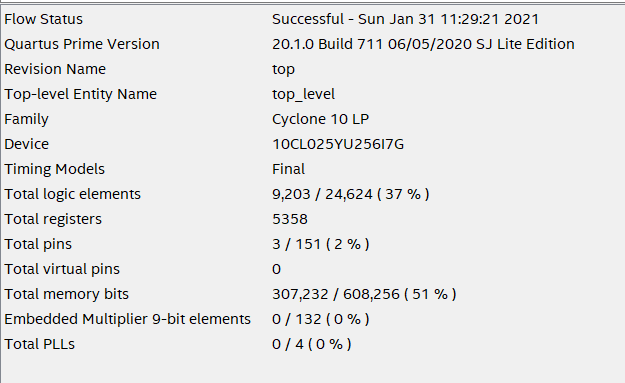
\includegraphics[width=\linewidth]{images/main_cyclone}
		\caption{Результат компиляции проекта}
		\label{fig:main_cyclone}
	\end{figure}

    \begin{figure}[H]
		\centering
		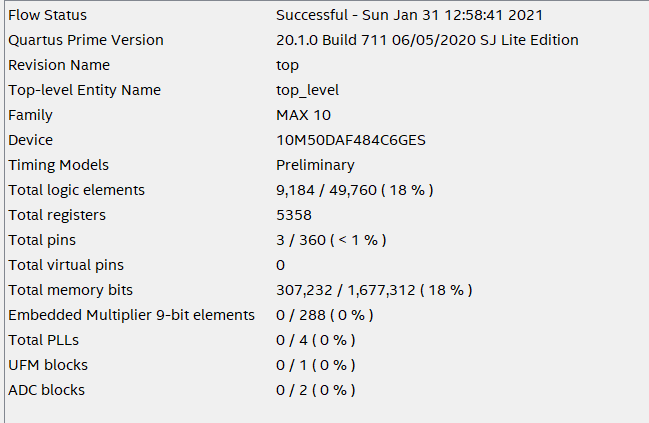
\includegraphics[width=\linewidth]{images/main_max10}
		\caption{Результат портирования проекта на MAX10}
		\label{fig:main_max10}
	\end{figure}

    \section{Самостоятельная работа}

   %   {\small \VerbatimInput{code/04_extra.txt}}


    \section{Исходные коды}

    Исходные коды доступны на \href{https://github.com/AsciiShell/hse_hlimds_labs}
    {https://github.com/AsciiShell/hse\_hlimds\_labs}.

    Pull request работы \href{https://github.com/AsciiShell/hse_hlimds_labs/pull/5}
    {https://github.com/AsciiShell/hse\_hlimds\_labs/pull/5}.


    \section{Выводы по работе}

    В ходе работы был изучены технологии создания многопроцессорных систем и взаимодействия между различными ядрами.

\end{document} % конец документа
